Play the message signal using
\begin{lstlisting}
sudo apt install ffmpeg
ffplay /fm/codes/msg/Sound_Noise.wav
\end{lstlisting}
\begin{enumerate}[label=\arabic*.,ref=\thesection.\theenumi]
\numberwithin{equation}{enumi}
\item Find the sampling rate of the message.
\item Plot the spectrum of the message signal using the builtin FFT algorithm.\\
	\solution		
\begin{figure}[H]
\centering
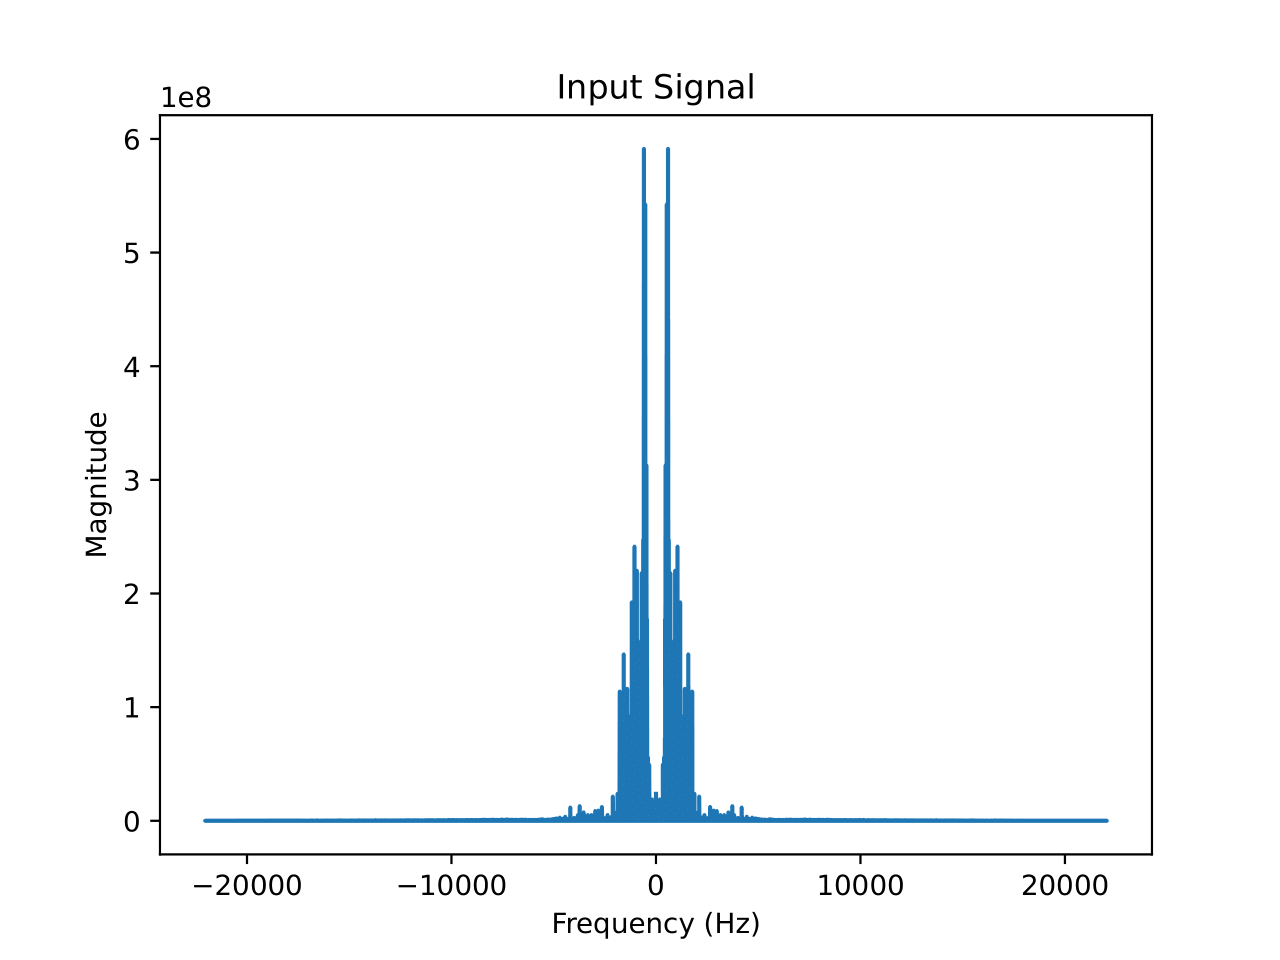
\includegraphics[width=\columnwidth]{fm/msg/figs/FFTbuiltin/inputs-1.png}
\caption{Plot of spectrum of message signal using builtin FFT algorithm.}
\label{fig:FFTb}
\end{figure}
\item Find the number of samples used to compute the FFT.
The folowing code plots the spectrum in \figref{fig:FFTb} using the builtin FFT algorithm of the python library 'Numpy.'
\begin{lstlisting}
/fm/codes/msg/msg_spec_amp.py
\end{lstlisting}
\item What does the following command do?
\begin{lstlisting}
f_i = np.fft.fftfreq(len(audio_data), d=1/sample_rate)
\end{lstlisting}

\item Plot the spectrum of the message signal by writing your own FFT algorithm.\\
	\solution
\begin{figure}[H]
\centering
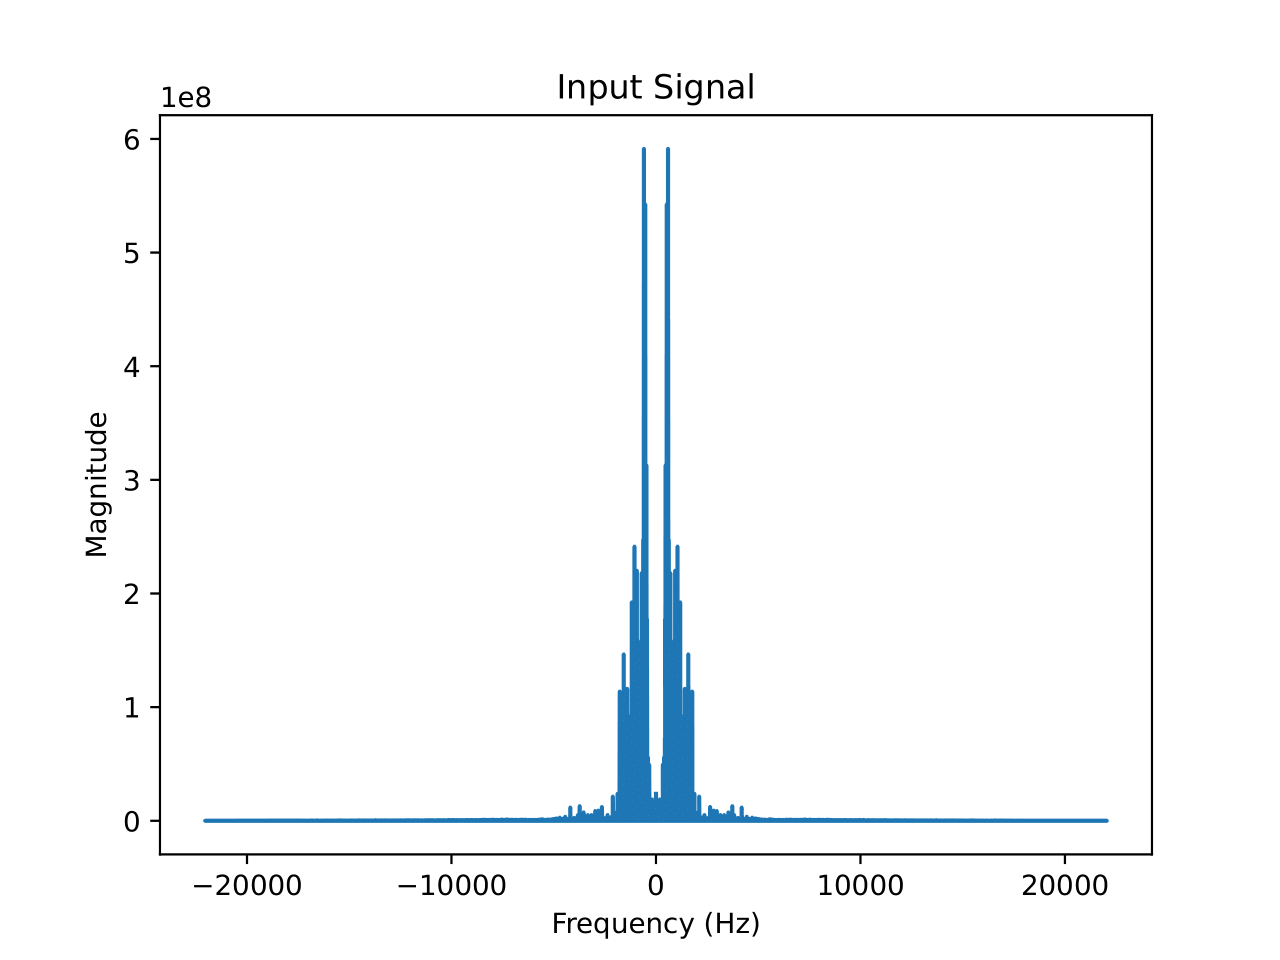
\includegraphics[width=\columnwidth]{fm/msg/figs/FFTown/input2.png}
\caption{Plot of spectrum of message signal using own FFT algorithm.}
\label{fig:FFTo}
\end{figure}
The folowing code plots the spectrum in \figref{fig:FFTo} using the DFT defined in  \eqref{eq:app-dft-def}.
\begin{lstlisting}
python3 fm/codes/msg/FFTmsg.py
\end{lstlisting}

\item Find the bandwidth of the message signal.\\
\solution First step is to calculate the bandwidth of message signal by computing Power Spectral density defined in \eqref{eq:app-psd-def} \\
Then set the threshold upto which the signal has significant frequencies.
After that eliminate insignificant frequencies using mask function defined in the code below\\
\begin{lstlisting}
/fm/codes/input.py
\end{lstlisting}
Now bandwidth can be calculated mathematically using the following formula:
\begin{align*}
B=mask_{maxi}-mask_{min}
\end{align*}
where $mask_{maxi}$ and $mask_{min} $ are the maximum amd minimum frequency bounds of the range  respectively.\\

\end{enumerate}
